\documentclass[../Matematyka.tex]{subfiles}

\begin{document}
\section{Rachunek prawdopodobieństwa i kombinatoryka}

\subsection{Elementy kombinatoryki}
\subsubsection{Symbol sumy}
\(\sum\) - sigma, symbol sumy
\[\sum^{5}_{i=2} i^2 = 2^2 + 3^2 + 4^2 + 5^2 = 4 + 9 + 16 + 25 = 54\]

\subsubsection{Symbol iloczynu}
\(\prod\) - pi, symbol iloczynu
\[\prod^{n}_{i=1} i = 1 \cdot 2 \cdot 3 \cdot \ldots \cdot n = n!\]

\subsubsection{Silnia}
\(n!\) - \(n\) silnia \(\qquad n \in \mathbb{N}_0\)

\begin{displaymath}
    n! =
    \begin{cases}
        1,                              & \quad n = 0 \lor n = 1 \\
        1 \cdot 2 \cdot \ldots \cdot n, & \quad n > 1
    \end{cases}
\end{displaymath}

\[n! = (n - 1)! \cdot n, \quad n \in \mathbb{N}\]

Def. Permutacja skończonego zbirou \(A\) to ciąg wszystkich elementów zbioru \(A\).\par
Tw. Ilość wszystkich permutacji zbioru \(n\)-elementowego wynosi \(n!\).

\subsubsection{Symbol Newtona}

\begin{align*}
    \binom{n}{k} =
    \frac{n!}{k!(n-k)!} \qquad &
    \substack{
    k,\;n\;\in\;\mathbb{N}_0     \\
        k\;\leq\;n
    }                            \\
    \binom{n}{n-k} =
    \binom{n}{k} \qquad        &
    \substack{
    k,\;n\;\in\;\mathbb{N}_0     \\
        k\;\leq\;n
    }
\end{align*}

\begin{displaymath}
    \binom{n}{0} = 1 \quad
    \binom{n}{1} = n \quad
    \binom{n}{n - 1} = n \quad
    \binom{n}{n} = 1
\end{displaymath}

Tw. Ilość wszystkich \(k\)-elementowych podzbiorów zbioru \(n\)-elementowego wynosi \(\binom{n}{k}\)\par
Tw. Ilość wszystkich podzbiorów zbioru \(n\)-elementowego \(2^n\)\par
Tw. Dla \(k, n \in \mathbb{N}, k \leq n\)
\begin{displaymath}
    \binom{n}{k-1}+
    \binom{n}{k} =
    \binom{n+1}{k}
\end{displaymath}

\subsubsection*{Dwumian Newtona}
Tw. Dwumian Newtona, dla  \(a, b \in \mathbb{R} \;\text{i}\; n \in \mathbb{N}\)

\[(a+b)^n = \sum^{n}_{k=0} \binom{n}{k}a^{n-k}b^k\]

\subsubsection*{Trójkąt Pascala}

\[\binom{0}{0}\]
\[\binom{1}{0}\quad\binom{1}{1}\]
\[\binom{2}{0}\quad\binom{2}{1}\quad\binom{2}{2}\]
\[\binom{3}{0}\quad\binom{3}{1}\quad\binom{3}{2}\quad\binom{3}{3}\]
\[\binom{4}{0}\quad\binom{4}{1}\quad\binom{4}{2}\quad\binom{4}{3}\quad\binom{4}{4}\]
\[\binom{5}{0}\quad\binom{5}{1}\quad\binom{5}{2}\quad\binom{5}{3}\quad\binom{5}{4}\quad\binom{5}{5}\]
\[\binom{6}{0}\quad\binom{6}{1}\quad\binom{6}{2}\quad\binom{6}{3}\quad\binom{6}{4}\quad\binom{6}{5}\quad\binom{6}{6}\]

\[1\]
\[1\quad1\]
\[1\quad2\quad1\]
\[1\quad3\quad3\quad1\]
\[1\quad4\quad6\quad4\quad1\]
\[1\quad5\quad10\quad10\quad5\quad1\]
\[1\quad6\quad15\quad20\quad15\quad6\quad1\]

\subsubsection{Regóła mnożenia}
Jeżeli pewien wybór zależy od skończenie wielu decyzji, powiedzmy \(k\),
przy czym podejmując pierwszą decyzję mamy \(n_1\) możliwości, drugą \(n_2\) możliwości,
\(\ldots\), \(k\)-tą \(n_k\) możliwości, bo wybór ten może być zrobiony na:

\[n = n_1 \cdot n_2 \cdot \ldots \cdot n_k\]

\subsubsection{Permutacja bez powtórzeń}
\textit{Permutacja bez powtórzeń} zbioru \(n\)-elementowego \(A = \{a_1, a_2, \ldots, a_n\}\), dla
\(n \in \N\) nazywamy każdy \(n\)-wyrazowy ciąg utworzony ze wszystkich \(n\)-elementów zbioru
\(A\), czyli każde uporządkowanie elementów zbioru \(A\).

Liczba wszystkich różnych permutacji bez powtórzeń zbioru \(n\)-elementowego jest równa
\[P_n = n!\]

Permutacje wykorzystujemy, gdy:
\begin{itemize}
    \item występują wszystkie elementy zbioru,
    \item kolejność jest istotna.
\end{itemize}

\subsubsection{Permutacja z powtórzeniami}
\textit{Permutacją \(n\)-wyrazową z powtórzeniami} zbioru \(k\)-elementowego
\(A = \{a_1, a_2, \ldots, a_k\}\), w której element \(a_i\) występuje \(n_i\) razy, \(i = 1, 2, \ldots, k\), przy czym \(\sum_{i=0}^{k}n_i = n\).

Liczba wszystkich różnych \(n\)-wyrazowych permutacji z powtórzeniami ze zbioru \(k\)-elementowego jest równa:
\[P_n(n_1, n_2, \ldots, n_k) = \frac{n!}{n_1! \cdot n_2! \cdot \ldots \cdots n_k!},\]
\[\text{gdzie } n_i \in \N, i=1,2,\ldots,k \text{, } n_i \text{ - liczba powtórzeń elementu } a_i \in A, \sum_{i=0}^{k}n_i = n\]

\subsubsection{Wariacja z powtórzeniami}
\textit{Wariacją \(k\)-wyrazową z powtórzeniami} zbioru \(A\), \(n\)-elementowego, gdzie \(k\in\N\),
nazywamy każdy \(k\)-wyrazowy ciąg, którego wyrazami są elementy danego zbioru \(A\).

Liczba wszystkich różnych \(k\)-wyrazowych wariacji z powtórzeniami zbioru \(n\)-elementowego jest równa:
\[W_n^k=n^k\]

Wariacje z powtórzeniami wykorzystujemy, gdy:
\begin{itemize}
    \item kolejność elementów jest istotna,
    \item elementy mogą się powtarzać (losowanie ze zwracaniem),
    \item niekoniecznie wszystkie elementy zbioru są wykorzystane.
\end{itemize}

\newpage
\subsubsection{Wariacja bez powtórzeń}
\textit{Wariacją \(k\)-wyrazową bez powtórzeń} zbioru \(A\), \(n\)-elementowego, gdzie \(k\in\N\),
nazywamy każdy \(k\)-wyrazowy ciąg różnowartościowy, którego wyrazami są elementy danego zbioru \(A\).

Liczba wszystkich różnych \(k\)-wyrazowych wariacji bez powtórzeń zbioru \(n\)-elementowego jest równa
\[V_n^k=\frac{n!}{(n-k)!}\]

Wariacje bez powtórzeń wykorzystujemy, gdy:
\begin{itemize}
    \item kolejność elementów jest istotna,
    \item elementy nie mogą się powtarzać (losowanie bez zwracania),
    \item niekoniecznie wszystkie elementy zbioru są wykorzystane.
\end{itemize}

\subsubsection{Kombinacja bez powtórzeń}
\textit{Kombinacją \(k\)-elemntową bez powtórzeń} zbioru \(A\), \(n\)-elementowego, gdzie \(k\in\N\),
nazywamy każdy podzbiór \(k\)-elementowy zbioru \(A\), przy czym elementy nie mogą się powtarzać.

Liczba wszystkich różnych kombinacji \(k\)-elementowych bez powtórzeń jest równa:
\[C_n^k=\binom{n}{k}=\frac{n!}{k!(n-k)!}\]
\[\mathcal{A}\]

\subsection{Prawdopodobieństwo klasyczne}
\begin{align*}
    \omega      & \text{ - zdarzenie elementarne,}                             \\
    \Omega      & \text{ - zbiór wszystkich zdarzeń elementarnych,}            \\
    A           & \text{ - zdarzenie losowe, } A \subset \Omega,               \\
    \mathcal{A} & \text{ - zbiór wszystkich zdarzeń losowych,}                 \\
    \emptyset   & \text{ - zdarzenie niemożliwe,}                              \\
    \Omega      & \text{ - zdarzenie pewne,}                                   \\
    A\prim      & \text{ - zdarzenie przeciwne, } A\prim = \Omega \setminus A, \\
\end{align*}

Rodzinę podzbiorów \(\mathcal{A}\) zbioru \(\Omega\) nazywamy algebrą zbiorów, jeżeli:
\begin{enumerate}[label=(\roman*)]
    \item \(A, B \in \mathcal{A} \implies A \cup B \in \mathcal{A}\),
    \item \(A, B \in \mathcal{A} \implies A \cap B \in \mathcal{A}\),
    \item \(A \in \mathcal{A} \implies A\prim = (\Omega \setminus A) \in \mathcal{A}\),
    \item \(\Omega \in \mathcal{A}, \emptyset \in \mathcal{A}\).
\end{enumerate}

\newpage
Prawdopodobieństwo \(P(A)\) to liczba przypisana zdarzeniu losowemu
\begin{enumerate}[label=(\roman*)]
    \item \(A \cap B = \emptyset \implies P(A \cup B) = P(A) + P(B)\),
    \item \(A \subset B \implies P(B \setminus A) = P(B) - P(A)\),
    \item \(P(A\prim) = 1 - P(A)\),
    \item \(P(\emptyset) = 0\), \(P(\Omega) = 1\),
    \item \(A \subset B \implies P(A) \leq P(B)\),
    \item \(P(A) \in [0,1]\),
    \item \(P(A \cup B) = P(A) + P(B) - P(A \cap B)\).
\end{enumerate}

W modelu klasycznym prawdopodobieństwa zakładamy, że zbiór \(\Omega\) jest skończony i wszystkie zdarzenia elementarne są jednakowo prawdopodobne.

Zdarzenia losowe to wszystkie podzbiory zbioru \(\Omega\) i prawdopodobieństwo określa się wzorem:
\[P(A) = \frac{|A|}{|\Omega|}, \qquad |x| \text{ - liczność zbioru }x\]

\subsection{Prawdopodobieństwo warunkowe}
\(P(A|B)\) - prawdopodobieństwo zdarzenia \(A\) pod warunkiem, że zaszło zdarzenie \(B\).
\[A,B \subset \Omega, \quad P(B) > 0\]
\[P(A|B) = \frac{P(A \cap B)}{P(B)}\]

\subsubsection{Prawdopodobieństwo całkowite}

\subsubsection*{Rozkład przestrzeni \(\Omega\) (układ zupełny)}
Zdarzenia \(B_1, B_2, \ldots, B_n\) tworzą rozkład przestrzeni \(\Omega\), jeżeli:
\begin{enumerate}[label=(\roman*)]
    \item \(B_1 \cup B_2 \cup \dots B_n = \Omega\)
    \item \(B_i \cap B_j = \emptyset\), dla \(i \neq j\), \(i,j = 1,2,\ldots,n\)
    \item \(P(B_i) > 0\), dla \(i = 1,2,\ldots,n\)
\end{enumerate}

\subsubsection*{Tw. Prawdopodobieństwo całkowite}
Jeżeli \(B_1, B_2, \ldots, B_n\) tworzą rozkłąd \(\Omega\), to dla dowolnego zdarzenia \(A \subset \Omega\):
\[P(A) = \sum_{i=1}^{n} P(A|B_i)P(B_i)\]

\subsubsection*{Tw. wzór Bayes'a}
Jeżeli \(B_1, B_2, \ldots, B_n\) tworzą rozkład \(\Omega\), to dla dowolnego \(k \in \{1, 2, \ldots, n\}\)
\[P(B_k|A) = \frac{P(A|B_k)P(B_k)}{P(A)}\]

\subsection{Niezależność zdarzeń}
Zdarzenia \(A\) i \(B\) są niezależne, jeżeli:
\[P(A \cap B) = P(A) \cdot P(B)\]

Zdarzenia \(A_1, A_2, \ldots, A_n\) są niezależne, jeżeli dla każdego \(k \leq n\) i dla każdego ciągu indeksów \(i_1, i_2, \ldots, i_k\),
gdzie \(1 \leq i_1 < i_2 < \dots < i_k \leq n\), zachodzi warunek:
\[P(A_{i_1} \cap A_{i_2} \cap \ldots \cap A_{i_k}) = P(A_{i_1}) \cdot P(A_{i_2}) \cdot \ldots \cdot P(A_{i_k})\]

Jeżeli zdarzenia \(A\) i \(B\) są niezależne oraz \(P(A) > 0\) i \(P(B) > 0\), to
\begin{align*}
    P(A|B) & = \frac{P(A \cap B)}{P(B)} = \frac{P(A) \cdot P(B)}{P(B)} = P(A) \\
    P(B|A) & = \frac{P(B \cap A)}{P(A)} = \frac{P(A) \cdot P(B)}{P(A)} = P(B)
\end{align*}

\subsection{Zmienna losowa jednowymiarowa}
Zmienną losową nazywamy funkcję \(X\) przyporządkowującą zdarzeniu elementarnemu dokładnie jedną liczbę rzeczywistą,
tj. \(X : \Omega \rightarrow \R\).
\[ \{X < a\} = \{\omega \in \Omega : X(\omega) < a\} \]
\[ \{X > a\}, \{X \geq a\}, \{X \leq a\}, \{X = a\}, \{X \in (-\infty, a\;]\}, \ldots \]

\begin{multicols}{2}
    \setlength{\columnseprule}{1pt}
    \subsubsection*{Dystrybuanta}
    Funkcja dystrybuanty zmiennej losowej \(X\) to funkcja \(F : \R \rightarrow [0, 1]\) określona wzorem:
    \[F(x) = P(X \leq x), \quad x \in \R\]

    Właściwości dystrybuanty:
    \begin{enumerate}[label=(\roman*)]
        \item \(F(x)\) jest niemalejąca,
        \item \(F(x)\) jest prawostronnie ciągła,
        \item \(\lim\limits_{x \to -\infty} F(x) = 0\),
        \item \(\lim\limits_{x \to \infty} F(x) = 1\),
    \end{enumerate}

    \subsubsection*{Funkcja przeżycia}
    Funkcja przeżycia zmiennej losowej \(X\) to funkcja \(S : \R \rightarrow [0, 1]\) określona wzorem:
    \[S(x) = P(X > x) = 1 - F(x), \quad x \in \R\]

    Właściwości funkcji przeżycia:
    \begin{enumerate}[label=(\roman*)]
        \item \(S(x)\) jest malejąca,
        \item \(S(x)\) jest prawostronnie ciągła,
        \item \(\lim\limits_{x \to -\infty} S(x) = 1\),
        \item \(\lim\limits_{x \to \infty} S(x) = 0\),
    \end{enumerate}
\end{multicols}
Dystrybuanta \(F(x)\) oraz funkcja przeżycia \(S(x)\) wyznaczają rozkład zmiennej losowej \(X\).

\newpage
\subsubsection{Zmienne losowe dyskretne (skokowe)}
Zmienna losowa \(X\) ma rozkład dyskretny, jeżeli zbiór jej wartośći jest skończony bądź przeliczalny.
\[\{x_i : i \in I\} \text{ - ciąg (skończony lub nieskończony) wszystkich wartości zmiennej losowej } X\]
\[p_i = P(X = x_i), \quad \sum_ip_i=1, \quad i \in I\]
\[\{(x_i, p_i): i \in I\} \text{ - rozkład zm. l. } X\]

\begin{table}[H]
    \centering
    \caption{Rozkład dyskretnej zmiennej losowej \(X\)}
    \begin{tabular}{c||c|c|c|c}
        \(x_i\) & \(x_1\) & \(x_2\) & \(\ldots\) & \(x_n\) \\
        \hline
        \(p_i\) & \(p_1\) & \(p_2\) & \(\ldots\) & \(p_n\)
    \end{tabular}
\end{table}

Dystrybuanta dyskretnej zmiennej losowej \(X\) to:
\[
    F(x) =
    \begin{cases}
        0,                   & x < x_1,             \\
        p_1,                 & x_1 \leq x < x_2,    \\
        p_1 + p_2,           & x_2 \leq x < x_3,    \\
        \vdots                                      \\
        \sum_{i=1}^{n-1} p_i & x_{n-1} \leq x < x_n \\
        1,                   & x \geq x_n
    \end{cases}
\]

\subsubsection{Zmienne losowe ciągłe}
Ciągła zmienna losowa \(X\), to zmienna losowa zdefiniowana za pomocą funkcji gęstości prawdopodobieństwa \(f(x)\).

Funkcja \(f:\R \rightarrow \R\) jest gęstością rozkładu zmiennej losowej \(X\), jeżeli dla dowolnych \(a, b \in \R\) takich, że \(a \leq b\) zachodzi warunek:
\[P(X \in [a, b]) = \int_{a}^{b}\!f(x)dx\]

Funkcja gęstości prawdopodobieństwa spełnia warunki:
\begin{enumerate}[label=(\roman*)]
    \item \(f(x) \geq 0, \quad x \in \R\)
    \item \(\displaystyle\int_{-\infty}^{\infty}\!f(x)dx = 1\)
\end{enumerate}

Dystrybuanta ciągłej zmiennej losowej \(X\) to:
\[F(x) = \int_{-\infty}^{x}\!f(t)dt, \quad f(x) = F\prim(x), \quad x \in \R\]

Zmienna losowa \(X\) ma rozkład ciągły, jeżeli posiada funkcję gęstości \(f(x)\).

\newpage
\subsubsection*{Parametry zmiennych losowych}
\[EX \text{ - wartość oczekiwana zm. l. } X\]
\[EX = \int_\Omega\!XdP\]

\begin{multicols}{2}
    \begin{center}
        Zm. l. dyskretna:
    \end{center}
    \[EX = \sum_{i \in I} x_ip_i\]

    \begin{center}
        Zm. l. ciągła:
    \end{center}
    \[EX = \int_{-\infty}^{\infty}\!xf(x)dx\]
\end{multicols}

Momenty rzędu \(n : n \in \N\) zmiennej losowej \(X\):
\begin{itemize}
    \item \makebox[2cm][l]{absolutny}   \(M_n = E|X|^n\)
    \item \makebox[2cm][l]{zwykły}      \(m_n = EX^n\)
    \item \makebox[2cm][l]{centralny}   \(\mu_n = E(X-m)^n, \quad \text{gdzie } m = EX\)
\end{itemize}

\begin{multicols}{2}
    \begin{center}
        Zm. l. dyskretna:
    \end{center}
    \begin{align*}
        M_n   & = \sum_{i \in I} |x_i|^np_i     \\
        m_n   & = \sum_{i \in I} (x_i)^np_i     \\
        \mu_n & = \sum_{i \in I} (x_i - m)^np_i
    \end{align*}

    \begin{center}
        Zm. l. ciągła:
    \end{center}
    \begin{align*}
        M_n   & = \int_{-\infty}^{\infty}\!|x|^nf(x)dx     \\
        m_n   & = \int_{-\infty}^{\infty}\!(x)^nf(x)dx     \\
        \mu_n & = \int_{-\infty}^{\infty}\!(x - m)^nf(x)dx
    \end{align*}
\end{multicols}

Jeżeli istnieje moment absolutny rzędu \(n\) zmiennej losowej \(X\), to istnieją wszystkie momenty rzędu \(k : k \leq n\) zm. l. \(X\).

Najważniejsze momenty zmiennej losowej \(X\):
\begin{itemize}
    \item \makebox[3cm][l]{\(m_1 = EX\)}         - wartość oczekiwana zm. l. \(X\)
    \item \makebox[3cm][l]{\(m_2 = EX^2\)}       - drugi moment zwykły zm. l. \(X\)
    \item \makebox[3cm][l]{\(\mu_2 = E(X-m)^2\)} - drugi moment centralny zm. l. \(X\)
    \item \makebox[3cm][l]{\(VarX = \mu_2\)}     - wariancja zmiennej losowej \(X\)
\end{itemize}

\[VarX = EX^2 - (EX)^2 = m_2 - m^2\]

\newpage
\begin{multicols}{2}
    [Własności wartości oczekiwanej \(EX\) i wariancji \(VarX\) (\(\alpha \in \R\)) :]
    \begin{center}
        Wartość oczekiwana:
    \end{center}
    \begin{enumerate}
        \item \(E(\alpha) = \alpha\)
        \item \(E(\alpha X) = \alpha EX\)
        \item \(E(X + Y) = EX + EY\)
        \item \(X \geq 0 \implies EX \geq 0\)
        \item \(X \geq Y \implies EX \geq EY\)
    \end{enumerate}

    \begin{center}
        Wariancja:
    \end{center}
    \begin{enumerate}
        \item \(Var(\alpha) = 0\)
        \item \(Var(\alpha X) = \alpha^2 VarX\)
        \item Jeżeli \(X\) i \(Y\) są niezależne to \(Var(X + Y) = VarX + VarY\)
        \item \(VarX \geq 0\)
        \item \(Var(X \pm \alpha) = VarX\)
    \end{enumerate}
\end{multicols}

Odchylenie standardowe zmiennej losowej \(X\):
\[\sigma_x = SD(X) = \sqrt{VarX}\]

\subsubsection*{Nierówność Czebyszewa}
Jeżeli \(X\) jest zmienną losową o wariancji \(VarX\) i wartości oczekiwanej \(EX\), to dla dowolnego \(\varepsilon > 0\) zachodzi nierówność:
\[P(|X - EX| > \varepsilon) \leq \frac{VarX}{\varepsilon^2}\]

\subsubsection{Wybrane rozkłady dyskretne}
\subsubsection*{Rozkład dwumianowy (Bernoulliego)}
Próba Bernoulliego - eksperyment losowy, który kończy się jednym z dwóch możliwych wyników, nazywanych (umownie) sukcesem i porażką.
\begin{align*}
    p & \text{ - prawdopodobieństwo sukcesu,} \quad p \in (0, 1) \\
    q & \text{ - prawdopodobieństwo porażki,} \quad q = 1 - p    \\
\end{align*}
Rozkład dwumianowy to n-krotne niezależne powtórzenie próby Bernoulliego.
\[S \sim B(n, p) \qquad n \in \N\]
\(S\) - liczba sukcesów w \(n\) próbach Bernoulliego.
\[P(S = k) = \binom{n}{k} p^k q^{n-k}, \quad k = 0, 1, 2, \ldots, n\]
\(P(S = k)\) - prawdopodobieństwo, że w \(n\) próbach sukces wystąpi \(k\) razy.
\[ES = np \qquad VarS = npq\]

\(N\) - najbardziej prawdopodobna liczba sukcesów w \(n\) próbach Bernoulliego.
\begin{enumerate}[label=(\roman*)]
    \item \makebox[4cm][l]{Jeżeli \((n+1)p \notin \N\), to} \(N = \lfloor (n+1)p \rfloor\)
    \item \makebox[4cm][l]{Jeżeli \((n+1)p \in \N\), to} \(N_1 = (n+1)p \text{ i } N_2 = N_1 - 1\)
\end{enumerate}

\newpage
\subsubsection*{Rozkład geometryczny}
\[T \sim Geo(p), \quad p \in (0,1) \quad q = 1 - p\]
\(T\) - czas oczekiwania na pierwszy sukces w nieskońonym schemacie Bernoulliego (numer próby, w której po raz pierwszy wystąpi sukces).

\[P(T=n) = q^{n-1}p, \quad n = 1,2,3,\ldots\]

\[ET = \frac{1}{p}, \quad VarT = \frac{q}{p^2}\]

\subsubsection*{Rozkład Poissona}
\[N \sim Poiss(\lambda), \quad \lambda > 0\]
\(N\) - liczba szkód zgłoszonych w jednostce czasu.

\[P(N = k) = \frac{\lambda^k}{k!}e^{-\lambda}, \quad k = 0,1,2,3,\ldots\]

\[EN = \lambda \qquad VarN = \lambda\]

\newpage
\subsubsection{Wybrane rozkłady ciągłe}
\subsubsection*{Rozkład jednostajny}
Rozkład jednostajny na przedziale \([a, b]\):
\[X \sim \mathcal{U}([a,b])\]

\begin{multicols}{2}
    \begin{center}
        Gęstość \(f(x)\)
    \end{center}
    \begin{tikzpicture}
        \begin{axis}[
                axis lines = left,
                ymin=0, ymax=0.8,
                xmin=0, xmax=4,
                xtick={1, 3},
                xticklabels={\(a\), \(b\)},
                ytick={1/(3-1)},
                yticklabels={\(\frac{1}{b-a}\)},
                samples=100,
                domain=0:4,
                width=0.9\linewidth,
                height=5cm
            ]
            \addplot [
                domain=0:1,
                samples=2,
                line width=2pt
            ]
            {0};
            \addplot [
                domain=1:3,
                samples=2,
                line width=0.6pt
            ]
            {1/(3-1)};
            \addplot [
                domain=3:4,
                samples=2,
                line width=2pt
            ]
            {0};
            \addplot[dashed] coordinates {(1,0) (1,0.5)};
            \addplot[dashed] coordinates {(3,0) (3,0.5)};
            \addplot[dashed] coordinates {(0,0.5) (1,0.5)};
        \end{axis}
    \end{tikzpicture}

    \[
        f(x) =
        \begin{cases}
            \frac{1}{b-a}, & x \in [a,b]    \\
            0,             & x \notin [a,b]
        \end{cases}
    \]

    \begin{center}
        Dystrybuanta \(F(x)\)
    \end{center}
    \begin{tikzpicture}
        \begin{axis}[
                axis lines = left,
                ymin=0, ymax=1.6,
                xmin=0, xmax=4,
                xtick={1, 3},
                xticklabels={\(a\), \(b\)},
                ytick={1},
                yticklabels={1},
                samples=100,
                domain=0:4,
                width=0.9\linewidth,
                height=5cm
            ]
            \addplot [
                domain=0:1,
                samples=2,
                line width=2pt
            ]
            {0};
            \addplot [
                domain=1:3,
                samples=2,
                line width=0.6pt
            ]
            {(x-1)/(3-1)};
            \addplot [
                domain=3:4,
                samples=2,
                line width=0.6pt
            ]
            {1};
            \addplot[dashed] coordinates {(3,0) (3,1)};
            \addplot[dashed] coordinates {(0,1) (3,1)};
        \end{axis}
    \end{tikzpicture}

    \[
        F(x) =
        \begin{cases}
            0,               & x < a       \\
            \frac{x-a}{b-a}, & x \in [a,b] \\
            1,               & x > b
        \end{cases}
    \]
\end{multicols}

\subsubsection{Rozkład wykładniczy}
\[T \sim Exp(\lambda), \quad \lambda > 0\]
\begin{multicols}{2}
    \begin{center}
        Gęstość \(f(x)\)
    \end{center}
    \begin{tikzpicture}
        \begin{axis}[
                axis lines = left,
                axis y line=middle,
                ymin=0, ymax=1.6,
                xmin=-1, xmax=5,
                xtick={0},
                xticklabels={0},
                ytick={1},
                yticklabels={\(\lambda\)},
                samples=100,
                domain=-1:5,
                width=0.9\linewidth,
                height=5cm
            ]
            \addplot [
                domain=-1:0,
                samples=2,
                line width=2pt
            ]
            {0};
            \addplot [
                domain=0:5,
                samples=100,
                line width=0.6pt
            ]
            {exp(-x)};
            \addplot[dashed] coordinates {(0,1) (5,1)};
        \end{axis}
    \end{tikzpicture}

    \[
        f(x) =
        \begin{cases}
            \lambda e^{-\lambda x}, & x \geq 0 \\
            0,                      & x < 0
        \end{cases}
    \]

    \begin{center}
        Dystrybuanta \(F(x)\)
    \end{center}
    \begin{tikzpicture}
        \begin{axis}[
                axis lines = left,
                axis y line=middle,
                ymin=0, ymax=1.6,
                xmin=-1, xmax=5,
                xtick={0},
                xticklabels={0},
                ytick={1},
                yticklabels={1},
                samples=100,
                domain=-1:5,
                width=0.9\linewidth,
                height=5cm
            ]
            \addplot [
                domain=-1:0,
                samples=2,
                line width=2pt
            ]
            {0};
            \addplot [
                domain=0:5,
                samples=100,
                line width=0.6pt
            ]
            {1-exp(-x)};
            \addplot[dashed] coordinates {(0,1) (5,1)};
        \end{axis}
    \end{tikzpicture}

    \[
        F(x) =
        \begin{cases}
            1 - e^{-\lambda x}, & x \geq 0 \\
            0,                  & x < 0
        \end{cases}
    \]
\end{multicols}
\subsubsection*{Własność braku pamięci rozkładu wykładniczego}
Jeżeli \(T\) ma rozkład wykładniczy, \(T \sim Exp(\lambda), \lambda > 0\) to dla dowolnych \(s, t > 0\)
\[P(T > s+t | T > s) = P(T > t)\]

\newpage
\subsubsection{Rozkład normalny}
\begin{multicols}{2}
    [\[X \sim \mathcal{N} (m, \sigma), \quad m \in \R, \sigma > 0\]]
    \begin{center}
        Gęstość
    \end{center}
    \[f_{m,\sigma}(x) = \frac{1}{\sqrt{2\pi} \sigma}e^{-\frac{(x-m)^2}{2\sigma^2}}, \quad x \in \R\]

    \begin{center}
        Dystrybuanta
    \end{center}
    \[\Phi_{m,\sigma}(x) = \int_{-\infty}^{x}f_{m,\sigma}(t)dt\]
\end{multicols}

\begin{center}
    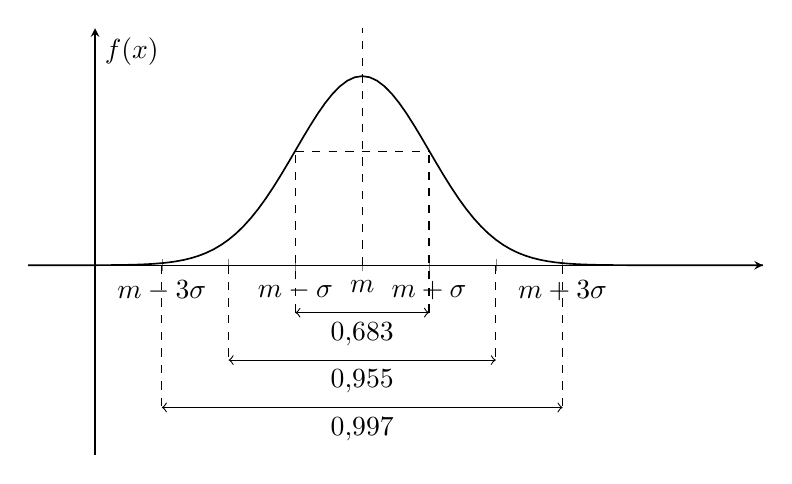
\begin{tikzpicture}
        \begin{axis}[
                axis lines = middle,
                ylabel = {\(f(x)\)},
                ymin=-0.4, ymax=0.5,
                xmin=-1, xmax=10,
                xtick={1, 2, 3, 4, 5, 6, 7},
                xticklabels={\(m-3\sigma\), ,\(m-\sigma\), \(m\), \(m+\sigma\), ,\(m+3\sigma\)},
                ytick={0},
                yticklabels={},
                samples=100,
                domain=-1:8,
                width=0.9\linewidth,
                height=7cm
            ]
            \addplot [
                domain=-1:10,
                samples=100,
                line width=0.6pt
            ]
            {1/(sqrt(2*pi)*1)*exp(-((x-4)^2)/(2*1^2))};
            \addplot[dashed] coordinates {(4,0) (4,0.5)};
            \addplot[dashed] coordinates {(3,-0.1) (3,0.24)};
            \addplot[dashed] coordinates {(5,-0.1) (5,0.24)};
            \addplot[dashed] coordinates {(3,0.24) (5,0.24)};
            \draw[<->] (axis cs:3, -0.1) -- (axis cs:5, -0.1) node[midway, below] {$0{,}683$};
            \addplot[dashed] coordinates {(2,0) (2,-0.2)};
            \addplot[dashed] coordinates {(6,0) (6,-0.2)};
            \draw[<->] (axis cs:2, -0.2) -- (axis cs:6, -0.2) node[midway, below] {$0{,}955$};
            \addplot[dashed] coordinates {(1,0) (1,-0.3)};
            \addplot[dashed] coordinates {(7,0) (7,-0.3)};
            \draw[<->] (axis cs:1, -0.3) -- (axis cs:7, -0.3) node[midway, below] {$0{,}997$};
        \end{axis}
    \end{tikzpicture}
\end{center}
\[EX = m \qquad VarX=\sigma^2 \qquad \sigma_x=\sigma\]

\subsubsection*{Rozkład normalny standardowy}
\[X \sim \mathcal{N} (0, 1)\]
\begin{multicols}{2}
    \begin{center}
        Gęstość
    \end{center}
    \[f(x) = \frac{1}{\sqrt{2\pi}}e^{-\frac{x^2}{2}}, \quad x \in \R\]

    \begin{center}
        Dystrybuanta
    \end{center}
    \[\Phi(x) = \int_{-\infty}^{x}f(t)dt = \frac{1}{\sqrt{2\pi}} \int_{-\infty}^{x}e^{-\frac{t^2}{2}}dt\]
\end{multicols}

\begin{center}
    \begin{tikzpicture}
        \begin{axis}[
                axis lines = middle,
                ylabel = {\(f(x)\)},
                ymin=-0.5, ymax=1.2,
                xmin=-5, xmax=5,
                xtick={-3, -2, -1, 0, 1, 2, 3},
                xticklabels={\(-3\), \(-2\), \(-1\), \(0\), \(1\), \(2\), \(3\)},
                ytick={1},
                yticklabels={\(1\)},
                samples=100,
                domain=-5:5,
                width=0.9\linewidth,
                height=8.5cm
            ]
            \addplot [
                domain=-5:5,
                samples=100,
                line width=0.6pt
            ]
            {1/(sqrt(2*pi)*1)*exp(-((x-0)^2)/(2*1^2))};
            \addplot[dashed] coordinates {(-1,-0.12) (-1,0.24)};
            \addplot[dashed] coordinates {(1,-0.12) (1,0.24)};
            \addplot[dashed] coordinates {(-1,0.24) (1,0.24)};
            \draw[<->] (axis cs:-1, -0.12) -- (axis cs:1, -0.12) node[midway, below] {$0{,}683$};
            \addplot[dashed] coordinates {(-2,0) (-2,-0.4)};
            \addplot[dashed] coordinates {(2,0) (2,-0.24)};
            \draw[<->] (axis cs:-2, -0.24) -- (axis cs:2, -0.24) node[midway, below] {$0{,}955$};
            \addplot[dashed] coordinates {(-3,0) (-3,-0.36)};
            \addplot[dashed] coordinates {(3,0) (3,-0.36)};
            \draw[<->] (axis cs:-3, -0.36) -- (axis cs:3, -0.36) node[midway, below] {$0{,}997$};
        \end{axis}
    \end{tikzpicture}
\end{center}

\[EX = 0 \qquad VarX=1 \qquad \sigma_x=1\]

\newpage
\subsection{Zmienne losowe dwuwymiarowe}
\[X,Y : \Omega \rightarrow \R \qquad Z = (X,Y) \text{ - wektor losowy}\]

\subsubsection{Tw. Nierówność Schwarza}
Jeżeli \(EX^2 < \infty\) i \(EY^2 < \infty\), to
\[|E(XY)| \leq \sqrt{EX^2 \cdot EY^2}\]

\subsubsection{Kowariancja}
Jeżeli \(EX^2 < \infty\) i \(EY^2 < \infty\), to kowariancja zmiennych losowych \(X\) i \(Y\) to liczba \(Cov(X,Y)\) określona wzorem:
\[Cov(X,Y) = E((X-EX)(Y-EY))\]

Tw. \(Cov(X,Y) = E(XY) - EX \cdot EY\)

Tw. \(|Cov(X,Y)| \leq \sigma_x \cdot \sigma_y\)

\subsubsection*{Współczynnik korelacji}
Jeżeli \(0 < VarX < \infty\) i \(0 < VarY < \infty\) to współczynnik korelacji liniowej zm. l. \(X\) i \(Y\) to liczba \(\varrho(X,Y)\) zadana wzorem:
\[\varrho(X,Y) = \frac{Cov(X,Y)}{\sigma_x \cdot \sigma_y}\]

\[-1 \leq \varrho(X,Y) \leq 1\]
\[\varrho(X,Y) \in [-1,1]\]

Załóżmy, że \(0 < VarX < \infty\) i \(0 < VarY < \infty\), wówczas:
\begin{enumerate}[label=(\roman*)]
    \item \makebox[2.1cm][l]{\(\varrho(X,Y) = 0\)} \(\iff X\) i \(Y\) są nieskorelowane
    \item \makebox[2.1cm][l]{\(\varrho(X,Y) > 0\)} \(\iff X\) i \(Y\) są dodatnio skorelowane
    \item \makebox[2.1cm][l]{\(\varrho(X,Y) < 0\)} \(\iff X\) i \(Y\) są ujemnie skorelowane
    \item \makebox[2.1cm][l]{\(\varrho(X,Y) = \pm 1\)} \(\iff X\) i \(Y\) są liniowo skorelowane
\end{enumerate}

Jeżeli \(\varrho(X,Y) = \pm 1\), to istnieją liczby \(a, b \in \R\) takie, że
\[Y = aX + b \qquad 
\substack{
    \text{Jeżeli } \varrho(X,Y) = 1 \text{, to } a > 0\\
    \text{Jeżeli } \varrho(X,Y) = -1 \text{, to } a < 0 
}\]

\(X\) i \(Y\) są nieskorelowane \(\iff Cov(X,Y) = 0\)

Fakt: \(X\) i \(Y\) są nieskorelowane \(\iff\) \(Cov(X,Y) = 0\)

Tw. Jeżeli \(EX^2 < \infty, \quad i = 1, 2, \ldots, n\), to
\[Var(\sum^{n} X_i) = \sum^{n} Var(X_i) + 2 \!\!\!\! \sum_{1 \leq i < j \leq n} \!\!\!\! Cov(X_i, X_j)\]

Tw. Jeżeli zmienne losowe \(X_1, X_2, \ldots, X_n\) są parami nieskorelowane, to
\[Var(\sum^{n} X_i) = \sum^{n} Var(X_i)\]

\subsubsection{Niezależne zmienne losowe}
Zmienne losowe \(X_1, X_2, \ldots, X_n\) są niezależne jeżeli dla dowolnych zbiorów borelowskich \(B_1, B_2, \ldots, B_n \subset \R\) zdarzenia \({X_1 \in B_1}, {X_2 \in B_2}, \ldots, {X_n \in B_n}\) są niezależne.

Tw. Jeżeli \(X_1, X_2, \ldots, X_n\) są niezależne oraz \(E|X_i|<\infty, i = 1, 2, \ldots, n\), to
\[E(\prod^n X_i) = \prod^n EX_i\]

Jeżeli \(X\) i \(Y\) są niezależne, to są nieskorelowane.

Tw. Jeżeli \(X_1, X_2, \ldots, X_n\) są niezależne, to
\[Var(\sum^n X_i) = \sum^n Var(X_i)\]

\subsubsection{Rozkłady niezależnych zmiennych losowych}
Tw. Jeżeli \(X\) i \(Y\) to niezależnie zmienne losowe o rozkładzie ciągłym z gęstościa \(f(x)\) i \(g(y)\) odpowiednio oraz \(S = X + Y\), to \(S\) ma ma również rozkład ciągły z gęstością \(h(x)\)
\[h(x) = \int f(t)g(x-t)dt, \quad x \in \R\]
\[h = f * g \qquad h \text{ -- splot funckji } f \text{ i } g\]

Tw. Jeżeli \(X\) i \(Y\) to niezależne zm. losowe o rozkładzie Poissona, \(X \sim Poiss(\lambda_1)\) i \(X \sim Poiss(\lambda_2)\) oraz \(S = X + Y\), to \(S\) ma również rozkład Poissona \(S \sim Poiss(\lambda)\), gdzie \(\lambda = \lambda_1 + \lambda_2\)

Tw. Jeżeli \(X\) i \(Y\) to niezależne zm. losowe o rozkładzie normalnym, \(X \sim \mathcal{N} (m_1, \sigma_1)\) i \(Y \sim \mathcal{N} (m_2, \sigma_2)\) oraz \(S = X + Y\), to \(S\) ma rozkład normalny \(S \sim \mathcal{N} (m, \sigma)\), gdzie \(m = m_1 + m_2\) i \(\sigma^2 = \sigma_1^2 + \sigma_2^2\)

Tw. Jeżeli \(X_1, X_2, \ldots, X_n\) to niezależne zmienne losowe o tym samym rozkładzie normalnym \(X_i \sim \mathcal{N} (m, \sigma)\) oraz
\begin{align*}
    S_n = \sum^n X_i \qquad& \text{ i }\qquad T_n = \frac{\displaystyle\sum^n X_i}{n}\\
    \text{to } S_n \sim \mathcal{N}(m_s, \sigma_s) \qquad& \text{ i } \qquad T_N \sim \mathcal{N} (m_t, \sigma_t) \text{, gdzie}\\
    m_s = m \cdot n, \sigma_s = \sigma\sqrt{n} \qquad& \text{ i } \qquad m_t=m, \sigma_t=\frac{\sigma}{\sqrt{n}}
\end{align*}

\newpage
\subsection{Prawa Wielkich Liczb}
\subsubsection{Prawa Bernoulliego}
Nieskończony ciąg prób Bernoulliego
\[X_i = \begin{cases}
    0,& \text{ w } i\text{-tej próbie porażka}\\
    1,& \text{ w } i\text{-tej próbie sukces}\\
\end{cases}\]

\begin{table}[H]
    \centering
    \begin{tabular}{c|c|c}
        \(x_i\) & \(0\) & \(1\) \\\hline
        \(p_i\) & \(q\) & \(p\) 
    \end{tabular}
    \[q = 1 - p\]
\end{table}

\[EX_i = 0q + 1p = p \qquad EX^2_i = 0^2q + 1^2p = p\]
\[VarX_i = EX^2_i - (EX_i)^2 = p - p^2 = pq \qquad \sigma_{X_i} = \sqrt{pq}\]

\(X_1, X_2, X_3, \ldots\) -- ciąg niezależnych zm. losowych o tym samym rozkładzie

\(S_n = \sum^n X_i\) -- liczba sukcesów w \(n\) próbach Bernoulliego

\(T_n = \frac{\sum^n X_i}{n}\) -- częstość sukcesów w \(n\) próbach Bernoulliego

Tw. Słabe Prawo Wielkich Liczb Bernoulliego

Dla każdego \(\varepsilon > 0\)
\[\lim_{n \rightarrow \infty} P(|T_n - p| \leq \varepsilon) = 1\]

Tw. Mocne Prawo Wielkich Liczb Bernoulliego
\[P(\lim_{n\rightarrow\infty} T_n = p) = 1\]

Tw, Mocne Prawo Wielkich Liczb Kołmogorowa

Załóżmy, że \(X_1, X_2, \ldots\) to ciąg niezależnych zmiennych losowych o tym samym rozkładzie ze skończoną wartością oczekiwaną \(EX_i = m, i=1,2,\ldots\)

Niech \(T_n = \frac{\sum^n X_i}{n}\) wówczas
\[P(\lim_{n\rightarrow\infty} T_n = m) = 1\]

\newpage
\subsection{Twierdzenia Graniczne}
\(X_1, X_2, X_3, \ldots\) -- niezależne zmienne losowe

\(S_n = \sum^n X_i\) -- suma

\(T_n = \frac{\sum^n X_i}{n}\) -- średnia

\(Z_n = \frac{S_n - ES_n}{SD(S_n)}\) -- standaryzowana suma

\[EZ_n = 0 \qquad VarZ_n = 1\]

\subsubsection*{Nieskończony ciąg prób Bernoulliego}
\[X_i = \begin{cases}
    0,& \text{ w } i\text{-tej próbie porażka}\\
    1,& \text{ w } i\text{-tej próbie sukces}\\
\end{cases} \qquad EX_i = p \quad VarX_i = pq\]

\(X_1, X_2, X_3, \ldots\) -- ciąg niezależnych zm. losowych o tym samym rozkładzie

\(S_n = \sum^n X_i\)

\(ES_n = np\)

\(VarS_n = npq\)

\(SD(S_n) = \sqrt{npq}\)

\(Z_n = \frac{S_n - np}{\sqrt{npq}}\)

Tw. Centralne Twierdzenie Graniczne de Moivre'a-Laplace'a

Jeżeli \(S_n\) to liczba sukcesów w \(n\) próbach Bernoulliego, to dla dowolnych \(a, b \in \R\) takich, że \(a < b\)
\[\lim_{n\rightarrow\infty} P(a \leq \frac{S_n - np}{\sqrt{npq} \leq b}) = \Phi(b) - \Phi(a)\]
gdzie \(\Phi\) to dystrybuanta \(\mathcal{N}(0,1)\).

Niech \(S_n\) to liczba sukcesów w \(n\) próbach Bernoulliego i \(T_n = \frac{S_n}{n}\) to częstość sukcesów w \(n\) próbach Bernoulliego, wówczas dla dużych \(n\) mamy:
\[Z_n \approx \mathcal{N}(0,1) \qquad S_n \approx \mathcal{N}(np, \sqrt{npq}) \qquad T_n \approx \mathcal{N}(p, \sqrt{\frac{pq}{n}})\]

Tw. Centralne Twierdzenie Graniczne Lindeberga-Levy'ego

Załóżmy, że \(X_1, X_2, X_3, \ldots\) to ciąg niezależnych zmiennych losowych o tym samym rozkładzie ze skończoną wariancją, \(EX_i = m, VarX_i=\sigma^2, i=1,2,\ldots\)

Niech \(S_n = \sum^n X_i\) i \(Z_n = \frac{S_n - ES_n}{SD(S_n)} = \frac{S_n - n \cdot m}{\sigma\sqrt{n}}\) oraz niech \(F_n(x)\) będzie dystrybuantą \(Z_n\). Wówczas dla każdego \(x \in \R\)
\[\lim_{n\rightarrow\infty}F_n(x) = \Phi(x)\]
\[\text{Wniosek: }\quad S_n \approx \mathcal{N}(m\cdot n, \sigma\sqrt{n}) \quad\text{ i }\quad T_n \approx \mathcal{N}(m, \frac{\sigma}{\sqrt{n}})\]

\subsubsection*{Sondaże (wielkość próby \(n\))}
Sondaż przeprowadzamy na grupie \(n\) osób. Jedno pytanie.

\(p\) -- procent osób w całej populacji, która odpowiada TAK.

\begin{multicols}{2}
    \[X_i \begin{cases}
        1, & i\text{-ty badany TAK}\\
        0, & i\text{-ty badany NIE lub NIE WIEM}
    \end{cases}\]

    \begin{table}[H]
        \centering
        \begin{tabular}{c|c|c}
            \(x_i\) & \(0\) & \(1\) \\\hline
            \(p_i\) & \(q\) & \(p\)
        \end{tabular}
    \end{table}
\end{multicols}

\(X_1, X_2, \ldots, X_n\) -- niezależne zm. losowe o tym samym rozkładzie

\(T_n = \frac{\sum^{n}X_i}{n}\) -- częstość odpowiedzi TAK w badaniu

Z CTG de Moivre'a-Laplace'a wynika, że
\[T_n \approx \mathcal{N}(p, \sqrt{\frac{pq}{n}})\]

Parametry badania:
\begin{itemize}
    \item \(n\) -- wielkość próby
    \item \(\varepsilon\) -- dopuszczalny błąd badania
    \item \(u\) -- poziom ufności
\end{itemize}

\[P(|T_n - p| \leq \varepsilon) \geq u\]
\[n \geq \frac{\alpha^2}{4\varepsilon^2} \qquad \text{gdzie } \Phi(\alpha) = \frac{1+u}{2}\]
\end{document}